\chapter{Results \& Discussion}\label{sec:results}

\begin{figure}[ht]
   \centering
   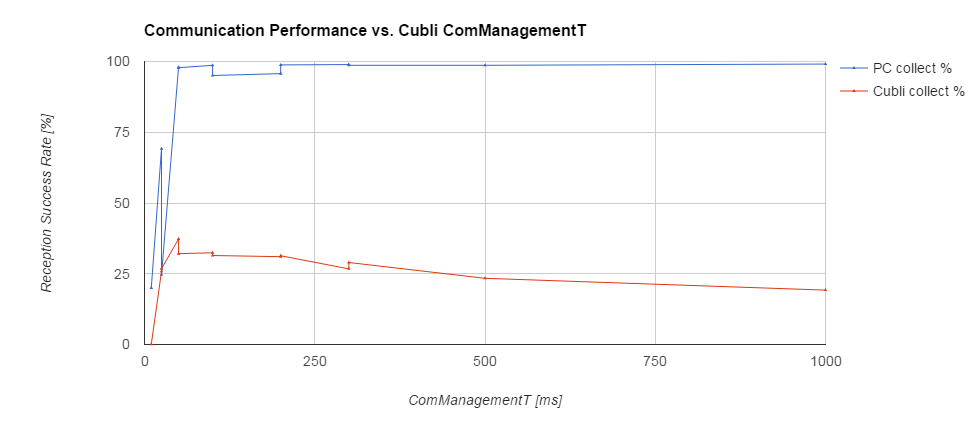
\includegraphics[width=1\textwidth]{img/comStats.png}
   \caption{A measure of the average communications success rate, with varying communication-update periods in cubli.}
   \label{img:comStats}
\end{figure}

As such we observe that on average, there is a 30\% chance of cubli collecting a message. This further means that if we are to send cubli the same message 5 times, the probability of at least one message being successfully received is ~85\% and for 10 identical messages, the same probability becomes ~97\% .\\

Another observed behavior during 